
\subsection*{Some complexity theory}
\addcontentsline{toc}{subsection}{Strongly asymetrical problems}

Sur la classification des problèmes en théorie de la complexité:\\


Définitions:\\
Classe L : un problème de décision est dans la classe L s'il peut être décidé
par un algorithme déterministe en un temps linéaire par rapport à la taille de l'instance.

Classe P : Un problème de décision est dans la classe P s'il peut être décidé sur une machine
déterministe en temps polynomial par rapport à la taille de la donnée, c'est la classe des 
problème pouvant être résolus en un temps polynomial: c'est la classe des problèmes dits facile

Classe NP\footnote{ NP est là pour "non-deterministic polynomial time" et non pour "non-polynomial time"} : La classe NP est formée des problèmes de décision qui ne peuvent être résolus en temps polynomial  que par un algorithme non déterministe; ou de manière plus informelle pour  c'est la classe des problèmes pour lesquels les seuls algorithmes connus de résolution (dc déterministe) sont ceux ayant une complexité exponentielle.\\ 
\\Définition:

On dit de manière générale, pour une classe de complexité C donnée, que un problème est dit C-difficile\footnote{Cette notion intuitive se définit plus formellement à l'aide de la notion de réduction polynomiale} s'il est plus dur à résoudre que tous les problèmes de C . Enfin un problème est C-Complet si et seulement si :
\begin{displaymath}
	\left\{
		\begin{array}{ll}
			\textrm{Il est dans C}\\
			\textrm{Il est C-difficile}\\
		\end{array} 			
	\right.
\end{displaymath}


\begin{figure}[h!]
\centering
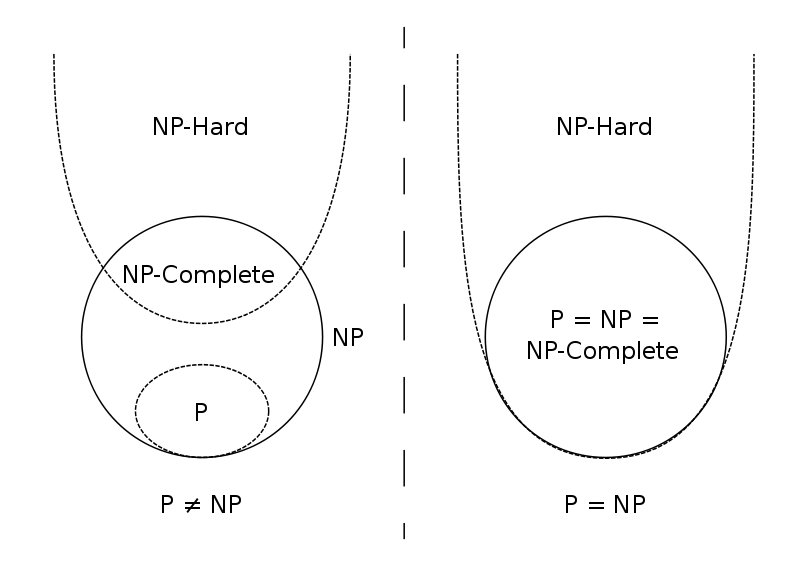
\includegraphics[width=70mm,height=50mm]{Pictures/NPcompleteNPhard.jpg}
\caption{Imbrication des classe de compléxités }
\end{figure}

On considère ici trois "problèmes difficiles", dont on précisera la difficulté en terme de classe de complexité, l'intérêt de cette partie est de souligner que "problème difficile" ne signifie pas "problème toujours difficile"
\begin{itemize}
	\item[] Problème 0: "du Sac a dos" ou Knapsack problem:
	 etant donnée une famille $(a_1, ..., a_p)$ une famille de p entiers positifs et un entier M, 
	 existe il une sous famille de $a_i$ de somme M.\\
	
	\item[] Problème 1: "plus court vecteur" ou SVP: Etant donnée une base B d'un sous réseau de V, 
	trouver un vecteur non nul de $\Gamma$ le plus court possible pour la norme Euclidienne.\\
	
	\item[] Problème 2: "plus proche vecteur" ou CVP: Etant donnée une base d'un sous réseau de V et un 
	vecteur  v $\in \mathbb{K}^{n}$ , trouver un vecteur u non nul de $\Gamma$ minimisant u-v pour la norme Euclidienne.\\
\end{itemize}

Théorème: Karp


Le problème du sac a dos est NP-Complet\\


Remarque importante: Quand il est prouvé qu'un problème appartient à une classe de complexité cela concerne le cas général, et rien ne dis qu'une classe d'instance particulière de ce problème ait la même complexité, d'ou l'importance de lier le pire cas au cas moyen ou de n'utiliser que des instances difficiles.
\begin{center}
	Pas de connections pire cas/moyen cas pour le problème du sac à dos\\ 
	$\mathit{ou \,\, la  \,\, chute  \,\, de  \,\, Merkle-Hellman :}$\\
\end{center}
1978 : Merkle-Hellman propose un crypto-système dont la sécurité est liée au problème du sac à dos\\ 
...et Merkle de proposer 100 dollars à quiconque casse son crypto-système.\\
1982 (voire 1979) : le système est cassé, en théorie seulement, par Shamir, qui gagne les 100 dollars.\\
1983 : Adleman le casse en pratique.\\
1984 : Brickell casse de multiples variantes de Merkle-Hellman, et gagne aussi 100 dollars.\\
1995 : la quasi-totalité des variantes sont cassées et plus personne ne croit plus en la possible utilité des sacs-à-dos.\\
Une percée -très- importante fut faite par Ajtai qui lia pour le SVP le pire cas au cas moyen.\\

Théorème : '1996 Ajtai:

Le problème SVP \footnote{on conjecture que le problème SVP est dans la classe NP ( donc qu'il est NP-complet )} du plus court vecteur pour la norme Euclidienne est NP-difficile pour une instance au hasard.
\begin{center}
Connection pire cas/moyen cas pour le SVP,\\ toutes les instances ont à peu près la même difficulté:\\ le SVP est NP-difficile pour une instance au hasard.\\
\end{center}

"SVP et ses variantes devraient toutes être considéré facile lorsque la dimension du réseau est inférieur a 70". 
\newpage

On termine cette section par une remarque importante:
\\
\\
\fbox{
\begin{minipage}{1\textwidth}
\begin{center}
Il n'existe actuellement aucun algorithme quantique connu\\
pouvant résoudre un problème NP-difficile de la géométrie des nombres. 
\end {center}
\end{minipage}
}